%%%%%%%%%%%%%%%%%%%%%%%%%%%%%%%%%%%%%%%%%
% Beamer Presentation
% LaTeX Template
% Version 1.0 (10/11/12)
%
% This template has been downloaded from:
% http://www.LaTeXTemplates.com
%
% License:
% CC BY-NC-SA 3.0 (http://creativecommons.org/licenses/by-nc-sa/3.0/)
%
%%%%%%%%%%%%%%%%%%%%%%%%%%%%%%%%%%%%%%%%%

%----------------------------------------------------------------------------------------
%	PACKAGES AND THEMES
%----------------------------------------------------------------------------------------

\documentclass[10pt]{beamer}

\mode<presentation> {

% The Beamer class comes with a number of default slide themes
% which change the colors and layouts of slides. Below this is a list
% of all the themes, uncomment each in turn to see what they look like.

%\usetheme{default}
%\usetheme{AnnArbor}
%\usetheme{Antibes}
%\usetheme{Bergen}
% \usetheme{Berkeley}
%\usetheme{Berlin}
%\usetheme{Boadilla}
%\usetheme{CambridgeUS}
% \usetheme{Copenhagen}
%\usetheme{Darmstadt}
%\usetheme{Dresden}
%\usetheme{Frankfurt}
%\usetheme{Goettingen}
%\usetheme{Hannover}
%\usetheme{Ilmenau}
%\usetheme{JuanLesPins}
%\usetheme{Luebeck}
% \usetheme{Madrid}
%\usetheme{Malmoe}
%\usetheme{Marburg}
\usetheme{Montpellier}
%\usetheme{PaloAlto}
%\usetheme{Pittsburgh}
%\usetheme{Rochester}
%\usetheme{Singapore}
%\usetheme{Szeged}
%\usetheme{Warsaw}

% As well as themes, the Beamer class has a number of color themes
% for any slide theme. Uncomment each of these in turn to see how it
% changes the colors of your current slide theme.

% \usecolortheme{albatross}
% \usecolortheme{beaver}
% \usecolortheme{beetle}
% \usecolortheme{crane}
% \usecolortheme{dolphin}
% \usecolortheme{dove}
% \usecolortheme{fly}
% \usecolortheme{lily}
% \usecolortheme{orchid}
% \usecolortheme{rose}
% \usecolortheme{seagull}
% \usecolortheme{seahorse}
% \usecolortheme{whale}
% \usecolortheme{wolverine}

%\setbeamertemplate{footline} % To remove the footer line in all slides uncomment this line
%\setbeamertemplate{footline}[page number] % To replace the footer line in all slides with a simple slide count uncomment this line

%\setbeamertemplate{navigation symbols}{} % To remove the navigation symbols from the bottom of all slides uncomment this line
}

\usepackage{graphicx} % Allows including images
\usepackage{booktabs} % Allows the use of \toprule, \midrule and \bottomrule in tables
% \usepackage{subcaption}
% \usepackage{float}
\usepackage[font=scriptsize]{subfig}
\usepackage[font=scriptsize,labelfont=bf]{caption}

\newcommand\toc{\begin{frame}
\tableofcontents[
  currentsection,
  sectionstyle=show/shaded,
  subsectionstyle=show/shaded/shaded
]
\end{frame}
}

\setbeamertemplate{headline}{}
\setbeamertemplate{navigation symbols}{}%remove navigation symbols
\setbeamertemplate{footline}[frame number]
\setbeamertemplate{bibliography item}{[\theenumiv]}
%----------------------------------------------------------------------------------------
%	TITLE PAGE
%----------------------------------------------------------------------------------------

\title[Comp 512 Project - Milestone 1]{Comp 512 Project - Milestone 1} % The short title appears at the bottom of every slide, the full title is only on the title page

\author{Jonah Caplan, HaiTong Yang - Group 28} % Your name
\institute % Your institution as it will appear on the bottom of every slide, may be shorthand to save space
{
McGill University \\ % Your institution for the title page
\medskip
\textit{jonah.caplan@mail.mcgill.ca,hai.yang@mail.mcgill.ca} % Your email address
}
\date{April 10, 2015} % Date, can be changed to a custom date

\begin{document}

\begin{frame}
\titlepage % Print the title page as the first slide
\end{frame}


\begin{frame}
\frametitle{System architecture}
\begin{itemize}
  \item Four resource managers are used: one for each type of reservable item and another for customer data.
\end{itemize}
\begin{figure}
\centering
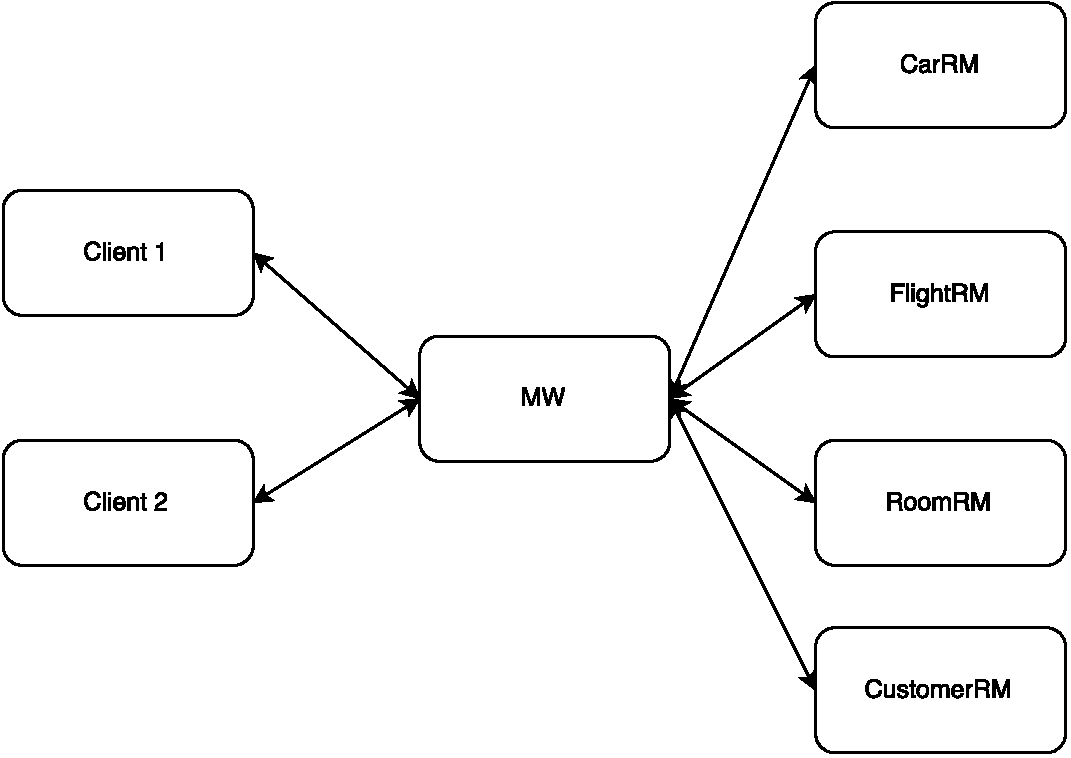
\includegraphics[scale=0.4]{figures/arch.pdf}
\end{figure}
\end{frame}

\begin{frame}
\frametitle{Reserving an itinerary}
\begin{figure}
\centering
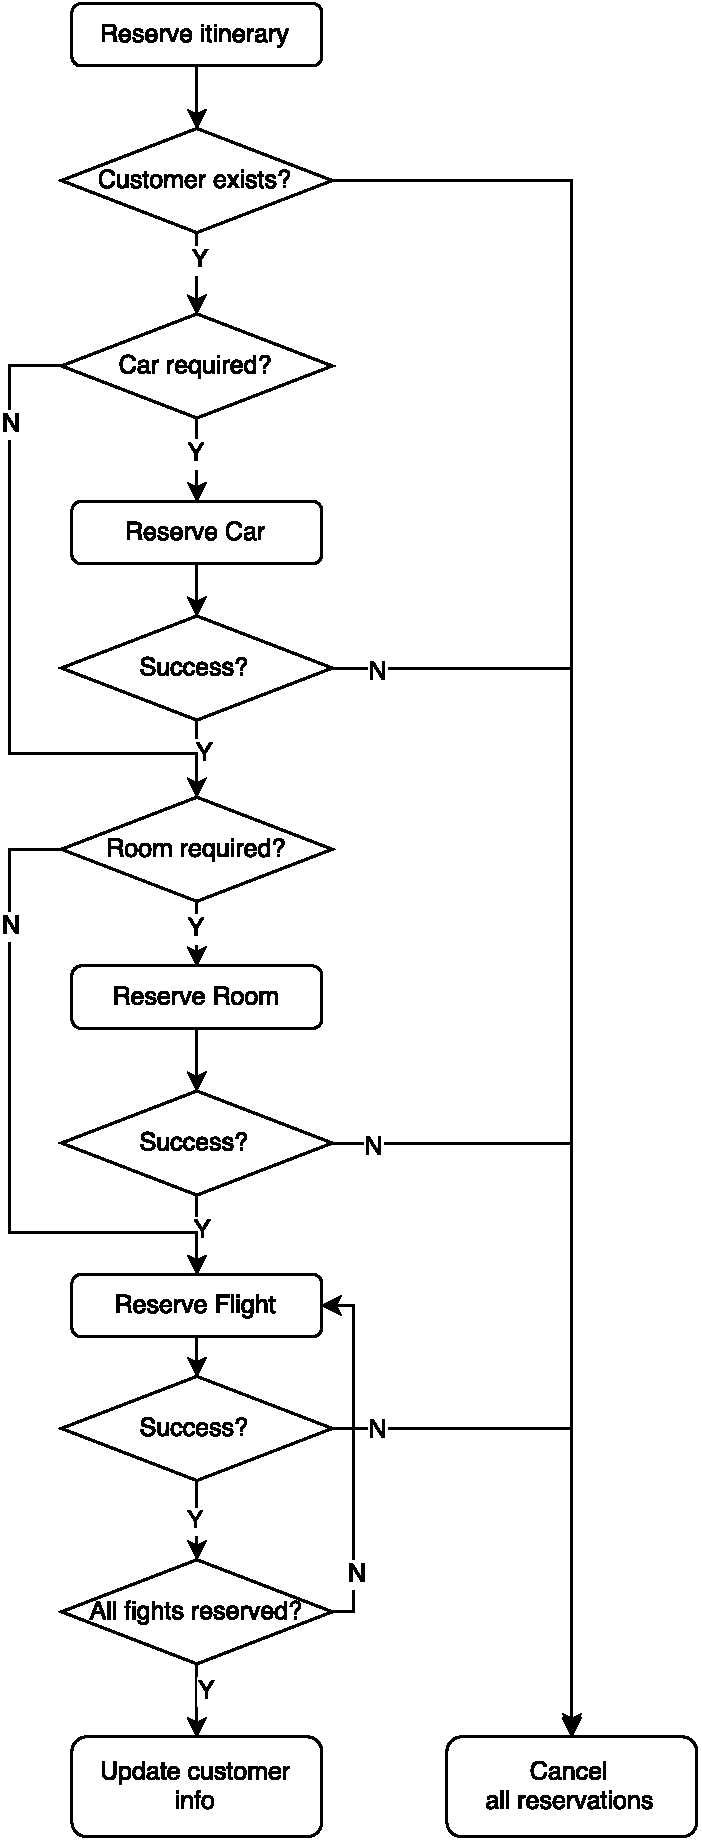
\includegraphics[scale=0.25]{figures/res-itin.pdf}
\end{figure}
\end{frame}

\begin{frame}
\frametitle{Thread management in TCP implementation}
\begin{figure}
\centering
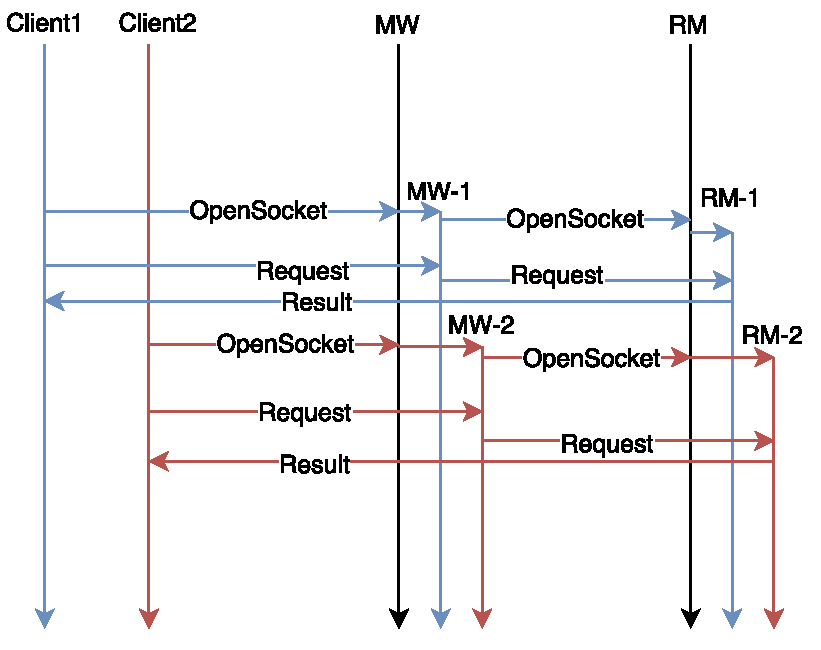
\includegraphics[scale=0.5]{figures/threads.pdf}
\end{figure}
\end{frame}


\begin{frame}
\frametitle{Parsing and thread creation in TCP server}
\begin{figure}
\centering
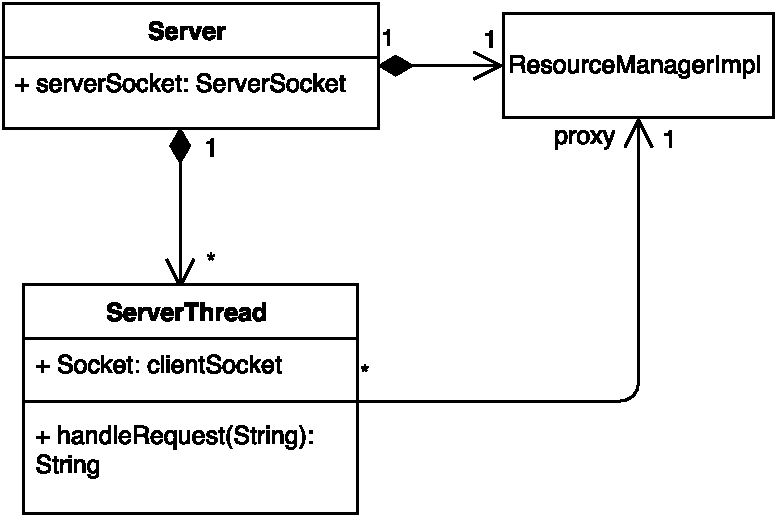
\includegraphics[scale=0.5]{figures/server-class.pdf}
\end{figure}
\end{frame}


\begin{frame}
\frametitle{Middleware TCP implementation}
\begin{figure}
\centering
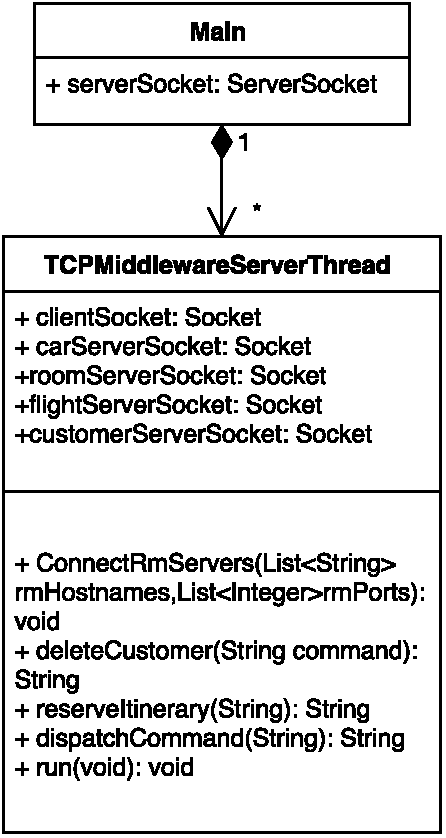
\includegraphics[scale=0.5]{figures/middleware-class.pdf}
\end{figure}
\end{frame}



\end{document} 
